\section{Software Overview}

\begin{figure}[ht!]
    \centering
    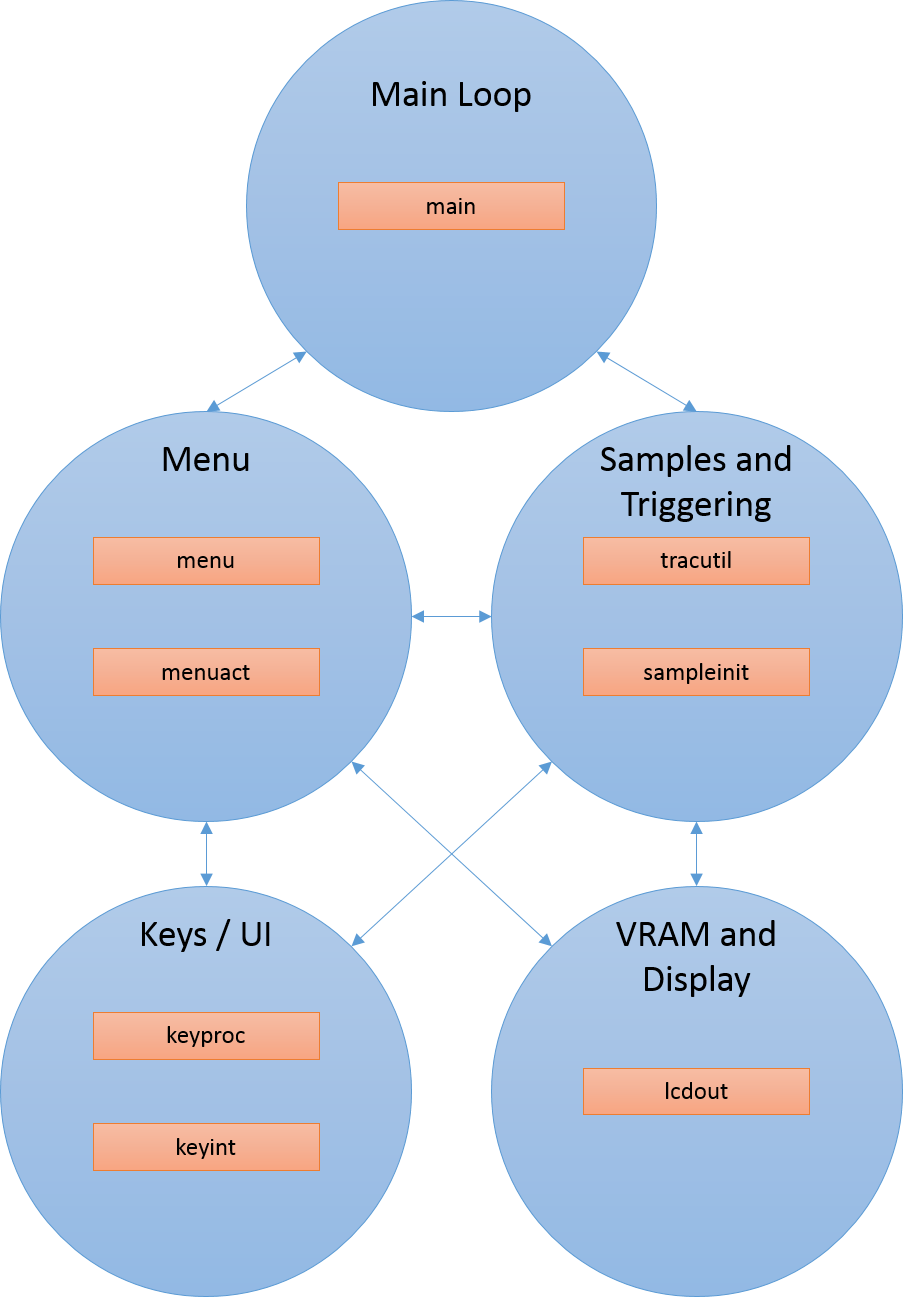
\includegraphics[width=3.5in]{block_diagrams/code.png}
		\caption{Software main components}
\end{figure}

\newpage

The software is composed of a number of separate files which can be grouped according to their like purposes. Consider the block diagram above.

The main loop continually checks for key presses and new samples in an infinite loop. The Menu subcomponent is responsible for displaying, updating, and keeping the state of the menu. The Samples and Triggering subcomponent is responsible for both collecting samples (\verb=sampleinit=) and displaying them (\verb=tracutil=). Both of these subcomponents utilize two other subcomponents, ``Keys/UI'' and ``VRAM and Display''. Keys is responsible for getting key interrupts and processing them, while VRAM and Display is responsible for handling the basics of writing to the display.

\section{Main Loop}
The main loop continually checks the three following things:
\begin{itemize}
	\item If ready to get another trace => do the trace
	\item If ready to display a trace => plot the trace
	\item If there's a key press => process the key
\end{itemize}

The only thing the main loop is responsible is installing the interrupt handlers during startup (these are the key interrupt handler and the adc interrupt handler).

\section{Menu}
There are two files of importance - \verb=menu= and \verb=menuact=. \verb=menu= provides functions related to the display of the menu, such as clearing and changing the selection on screen. \verb=menuact= provides functions related to what happens when certain menu actions are triggered, such as increasing the trigger level when so desired.

\section{Samples and Triggering}
Again, there are two files of importance - \verb=tracutil= and \verb=sampleint=. \verb=tracutil= will display a provided sample on the screen. In particular, the function \verb=plot_trace= handles the actual plotting of a new trace. In fact, it takes an array of sample buffers, one for each of the inputs (A, B, Logic analyzer).

On the other hand \verb=sampleint= is responsible for handling interrupts generated by the FPGA logic when a trigger occurs. When this happens, the FIFO sample data is read to a memory buffer, which the CPU (with \verb=tracutil=) can then plot.

\section{Keys / UI}
Once again, there are two files of importance - \verb=keyproc= and \verb=keyint=. \verb=keyproc= takes a given key code and determines what action it should take. This generally includes modifying the menu and changing one of the trigger control values (level, delay, etc).

\verb=keyint= is responsible for handling interrupts that are generated when a keypress event occurs. When handling such an interrupt, \verb=keyint= may either pass on that key code for \verb=keyproc= to take care of, or it may trigger the action itself. Typically, the pushbuttons below the display will trigger \verb=keyint= to pass on the key code to \verb=keyproc=, whereas the hardware mimic buttons trigger direct actions. This is because the hardware mimic buttons should not modify the menu.

\section{VRAM and Display}
There's one file of importance - \verb=lcdout=. This file includes functions for modifying the display, such as clearing, drawing a line, or writing a character or string. These functions are used by \verb=menu= for, for example, writing the menu text. \verb=tracutil= uses VRAM and Display functions (namely, \verb=plot_pixel=) for plotting the trace.
